\chapter{Анализ влияния алгоритма управления приводами на величину некомпенсированных моментов, возникающих при перенацеливании}\label{ch:ch2}
\section{Описание объекта исследования}\label{sec:ch2/sec1}

Одним из объектов исследования является модуль направленного обзора (МНО). Конструкция МНО предусматривает возможность поворота оси 
визирования по двум осям в пределах ограниченного угла. При этом оптическая 
система МНО разделена на две части. В подвижную часть входит зеркальный блок состоящий из главного зеркала  и вторичного зеркала , а неподвижная часть включает линзовый компенсатор и сканирующее зеркало. Оптические оси этих двух частей составляют угол $90^\circ \pm \beta$, где $\beta$-угол поворота зеркального блока по оси $OZ$ . Зеркальный блок имеет также возможность вращаться по оси $OY$ на угол $\alpha$. Связь частей оптической системы друг с другом осуществляется с помощью плоского сканирующего зеркала, развёрнутого относительно оси $ОХ$ на угол $45^\circ \pm \frac{\beta}{2}$.Таким образом, конструктивно подвижная часть установлена в кардане и имеет две степени свободы. Для изменения пространственной ориентации оси визирования МНО.


%\begin{figure}[ht]
%	\begin{minipage}[b][][b]{0.49\linewidth}\centering
%		\includegraphics[width=1\linewidth]{ypk} \\ б)
%	\end{minipage}
%	\hfill
%	\begin{minipage}[b][][b]{0.49\linewidth}\centering
%		\includegraphics[width=1\linewidth]{ypk_cut} \\ %б)
%	\end{minipage}
%	\caption{Система узкопольного канала}
%	\label{fig:ypk-pic}
%\end{figure}
Изменение пространственной ориентации оси визирования МНО осуществляется за счёт работы специальных приводов, которые поворачивают зеркальный блок относительно космического аппарата на углы $\alpha$ и $\beta$.
Приводы прикладывают к осям карданова подвеса соответствующие моменты для реализации углового перемещения зеркального блока. В соответствии с третьим законом Ньютона, к КА будут приложены равные, но противоположно направленные моменты в месте крепления приводов. Эти моменты называются реактивными.

Реактивные моменты, будучи приложенными к КА, приводят к дополнительному перемещению КА в пространстве, меняя направление оси визирования МНО, закреплённого на КА. Для стабилизации КА в полёте и удержании его на орбите используются гиродины (специальные маховики с приводами или двухстепенные гироскопы). Действие значительных по величине реактивных моментов приводит к существенным нагрузкам на гиродины, и к изначальному угловому положению КА можно вернуться лишь после продолжительного по времени переходного процесса всей системы стабилизации КА \cite{углова2019оценка, zhao2023effect}.

В представленной конструкции компенсация реактивного момента реализована за счёт установки маховика на оси двигателя через редуктор. Такое решение одновременно формирует противодействующий момент и обеспечивает автоматическую синхронизацию его вращения с движением нагрузки. При работе привода зеркального блока двигатель через редуктор передаёт вращение как на сам блок, так и на маховик, который разворачивается в противоположную сторону. В результате создаётся момент, равный по величине и противоположный по знаку моменту, приложенному к основанию от движения блока зеркал. Ключевым достоинством выбранной схемы является то, что синхронизация достигается конструктивно, без необходимости в отдельной системе управления маховиком или в алгоритмах согласования его работы с зеркальным блоком. Это существенно упрощает управление и повышает надёжность устройства. Дополнительное преимущество даёт применение редукторной кинематической связи: эквивалентный момент инерции маховика уменьшается пропорционально квадрату коэффициента передачи $i$, что позволяет снизить его массу при сохранении требуемого компенсирующего воздействия. Такой подход делает возможной эффективную компенсацию реактивного момента без значительного увеличения массы и энергопотребления, что особенно важно при проектировании компактных высокоточных приводов.Использование шагового двигателя дополнительно расширяет функциональные возможности конструкции. Так как вращение маховика жёстко связано с движением зеркального блока, управление углом поворота может осуществляться дискретно, по числу шагов двигателя. Это позволяет отказаться от отдельного датчика угла поворота блока зеркал и использовать управление «по шагам» как резервный режим в случае отказа основной системы обратной связи. Такая особенность повышает отказоустойчивость системы при сохранении требуемой точности задания углового положения.

Другим объектом исследования является оптико-механическая система (ОМС), представляющая собой зеркало с двумя степенями свободы.

\begin{figure}[ht] 
	\centerfloat{
		\includegraphics[scale=0.8]{zerkalo} 
	}
	\legend{1 – оптико-механическое устройство; 2 – рама несущая; 3 – привод редукторный OY; 4 – узел датчика угла; 5 – узел привода редукторного OZ; 6 – привод редукторный OZ; 7 – арретир технологический; 8 – технологический электронный блок управления ПЭС}
	\caption{Оптическая система Зеркало.}
	\label{fig:zerkalo} 
\end{figure}

Изделие, показанное на рисунке~\cref{fig:zerkalo}, представляет собой оптико-механическое устройство (ОМУ) (1) с поворотной электромеханической системой (ПЭС) и технологическим электронным блоком управления ПЭС (8), которые обеспечивают:
\begin{itemize}[beginpenalty=10000] % https://tex.stackexchange.com/a/476052/104425
	\item угловые перемещения ОМУ по двум координатам, позволяющие осуществить вращение линии визирования;
	\item высокую точность перемещения;
	\item малое значение остаточных реактивных моментов, действующих на основание при перенацеливании изделия;
	\item фиксирование пространственного положения линии визирования после завершения перенацеливания;
	\item стойкость к внешним воздействующим факторам.
\end{itemize}

ОМУ изделия состоит из зеркала, системы крепления и оси для установки в изделие.Зеркало выполнено из легковесного сплава, имеет монолитную конструкцию с шестигранными облегчающими выборками, гнездом под систему крепления и отверстия для размещения оси. Плоская рабочая поверхность зеркала сформирована оптической обработкой непосредственно поверхности легковесного сплава без применения дополнительного зеркального покрытия.

Система крепления и ось вращения обеспечивают надёжное крепление зеркала в ПЭС.

Конструктивно в состав ПЭС входят:
\begin{itemize}[beginpenalty=10000] % https://tex.stackexchange.com/a/476052/104425
	\item рама несущая (2);
	\item привод редукторный \textit{OZ} (3);
	\item узел датчика угла (4);
	\item узел привода редукторного \textit{ОY} (5);
	\item формирование сигналов оперативного и телеметрического контроля (ОК и ТМ);
\end{itemize}
Рама несущая (2) представляет собой жёсткую конструкцию в виде несущих опор, предназначенную для крепления всех составных частей изделия.

Привод редукторный \textit{OZ} (3) поворачивает зеркало ОМУ (1) вокруг вертикальной оси \textit{OZ}, обеспечивая перенацеливание по азимуту на углы до $\pm10^{\circ}$ . 
В состав привода редукторного \textit{OZ} входят два шаговых двигателя (основной и резервный) с волновым редуктором и маховиком.
Шаговые двигатели соединены друг с другом зубчатой передачей с коэффициентом передачи 1.

Каждый двигатель имеет два выходных вала с противоположных сторон двигателя. На один вал основного двигателя крепится маховик. На другой, через муфту и ось, – волновой редуктор, предназначенный для передачи вращения от шагового двигателя к системе крепления зеркала ОМУ (1). При этом выходной вал волнового редуктора вместе с зеркалом ОМУ вращается в направлении, обратном вращению валов основного двигателя, что обеспечивает вращение маховика в направлении, обратном вращению зеркала, и компенсацию момента, приложенного к основанию, возникающего при вращении зеркала.

К приводу редукторному \textit{OZ} крепится узел датчика угла (4), включающий преобразователь угловых перемещений, передающий информацию о текущем угле поворота зеркала по азимуту (вокруг оси \emph{OZ}).
Узел привода редукторного \emph{OY} (5) является подвижной частью изделия. В его состав входит поворотная несущая конструкция, состоящая из пластин и кронштейнов, с закреплённым на ней приводом редукторным \emph{OY} (6). 

Привод редукторный \emph{OY} поворачивает зеркало ОМУ вокруг горизонтальной оси \emph{OY}, обеспечивая перенацеливание по углу места на углы до $\pm10^{\circ}$. 

Узел датчика угла (4), установленный на оси ОМУ (1) с противоположной стороны от привода редукторного OY (6), обеспечивает измерение угла поворота зеркала по углу места (вокруг оси \emph{OY}).

Конструктивно привод редукторный \emph{OY} (6) и привод редукторный \emph{OZ} (3) выполнены одинаково и отличаются только маховиками. Конструкция датчиков угла, установленных по осям \emph{OY} и \emph{OZ}, также одинакова.

В составе изделия узел привода редукторного \emph{OY} обеспечивает также крепление ОМУ (1) и привода редукторного \emph{OZ} (3), и с помощью последнего вращается вокруг оси \emph{OZ} относительно рамы несущей (2). При этом привод редукторный \emph{OZ} (3) остаётся неподвижным, а привод редукторный \emph{OY} (6) разворачивается вместе с узлом привода редукторного \emph{OZ} (5) и зеркалом ОМУ. 

Технологический электронный блок управления (ТЭБУ) ПЭС (8) предназначен для управления ПЭС изделия по командам, поступающим извне от автоматизированной системы контроля и управления (АСКУ) в составе технологического стенда проверки основных параметров ПЗС ОМС.

Третьим объектом исследования является оптико-механический сканер, предназначенный для формирования развертки изображения на фотоприёмное устройство, работающее в режиме временной задержки и накопления (ВЗН). Сканер обеспечивает последовательное считывание изображения путём возвратно-вращательного движения плоского зеркала, расположенного в параллельном ходе лучей.Кинематическая схема сканера включает сканирующее зеркало и маховик компенсации, установленные на соосных валах. Для снижения влияния реактивных моментов, возникающих при перемещении зеркала, маховик разворачивается во встречном направлении, обеспечивая компенсацию приложенного к основанию момента. Такое решение минимизирует воздействие на космическую платформу и уменьшает нагрузку на систему стабилизации аппарата.Сканирующее зеркало выполнено из легковесного сплава и закреплено в оправе на трёх точках, что обеспечивает статическую определённость и равномерное распределение нагрузок. Для уменьшения массы при сохранении жёсткости тыльная сторона зеркала выполнена ячеистой. Поворот зеркала осуществляется моментным электродвигателем с постоянными магнитами, обеспечивающим высокую линейность и стабильность момента. Для синхронизации движения зеркала с опросом линейного фотоприёмного устройства сканер оснащён бесконтактным интерферометрическим датчиком углового положения, выполненным по схеме интерферометра Майкельсона с лазерным источником излучения. Такой датчик обеспечивает высокое разрешение измерения угла и гарантирует равномерность развёртки изображения.Для повышения коэффициента полезного действия сканирования и снижения энергопотребления в моменты реверса используются магнитные рекуператоры. Они аккумулируют кинетическую энергию системы «зеркало–маховик» и возвращают её в привод, что снижает тепловые и электрические потери. Дополнительно установлены бесконтактные концевые датчики на основе эффекта Холла, контролирующие пределы перемещения зеркала и маховика.


\section{Математическое описание реактивных моментов, возникающих при перенацеливании оптической системы МНО}\label{sec:ch2/sec2}

Особенностью конструкции МНО является несовпадение точки пересечения осей карданова подвеса с центром тяжести подвижного зеркального блока (Рисунок ~\cref{fig:tikz_YPK}).
Обозначим расстояние между этими точками за $r$. 

Рассмотрим результат воздействия реактивных моментов на основание с учётом расположения центра вращения карданова подвеса МНО относительно центра тяжести КА.
\begin{figure}[ht]
	\centerfloat{
		\ifdefmacro{\tikzsetnextfilename}{\tikzsetnextfilename{tikz_example_compiled}}{}% присваиваемое предкомпилированному pdf имя файла (не обязательно)
		
	\begin{tikzpicture}[scale=1.6, >=stealth, font=\LARGE]
%X0Y0Z0 axis
\draw [->, very thick] (13.75,13.25) -- (13.75,16.25)node[above] {$Y_0$};
\draw [->, very thick] (13.75,13.25) -- (11.5,11.5) node[above left] {$X_0$};
\draw [->,very thick] (13.75,13.25) -- (11.25,13.75) node[above] {$Z_0$};
\node at (13.85, 13.05) {$0_0$};
%Z0 line
\draw [thin, short] (11.25,13.75) -- (16.25,12.75);
%Z line
\draw [thin, short] (13.75,13.25) -- (16.75,13);

%X0Y0Z0 axis proection
\draw [thin] (10,8.25) -- (10,10.75) node[above] {$Y_0$};
\draw [thin] (10,8.25) -- (7.5,8.75) node[above] {$Z_0$};
\draw [thin] (10,8.25) -- (7.5,6.5) node[above left] {$X_0$};


%proection Z0 line
\draw [thin, short] (7.5,8.75) -- (12.5,7.75);
\draw [line width=0.9pt, ->,] (10,8.25) -- (10,10) node[right] {$M_{da}$};
%OXYZ axis
\draw [ ->, very thick] (10,8.25) -- (9.75,6.25) node[left] {$X$};
\draw [->, very thick] (10,8.25) -- (9.32, 10.2) node[above] {$Y$};
\draw[thick,->] (10, 10) arc[start angle=5,end angle=175,x radius=0.3cm, y radius=0.2cm];
\node at (9.7, 10.3) {$\beta$};
\draw [ ->, very thick] (10,8.25) -- (7,8.5) node[above] {$Z$};
\node at (10.20,8.33) {$0$};
\draw[thick,->] (8.8,8.5) arc[start angle=0,end angle=85,radius=-1.2cm];
\node at (9.5, 7.5) {$\alpha$};
%red line
\draw [ color={rgb,255:red,245; green,0; blue,0}, line width=1.6pt, short] (13.75,13.25) -- (10,8.25);
\node at (11, 10)[text=red] {$R$};
\draw [ color=red, line width=0.2pt, ->,] (10,8.25) -- (9.75,9)node[left] {$F_b$};



\draw [line width=0.9pt, ->,] (10,8.25) -- (7.8,8.43) node[below] {$M_{db}$};
\draw [ color=red, line width=0.2pt, ->,] (10,8.25) -- (8.5,8.37) node[below] {$F_a$};
%blue circle
\draw [ color={rgb,255:red,4; green,45; blue,251} , fill={rgb,255:red,45; green,166; blue,240}, line width=0.2pt ] (9.83,7) circle (0.25cm);



\draw [ color=blue, very thick, short] (10,8.25) -- (9.83,7);
\node at (10, 7.5)[text=blue] {$r$};
		\end{tikzpicture}
		
	}
	\legend{}
	\caption[Пример \texttt{tikz} схемы]{Смещение центра масс блока зеркал МНО}\label{fig:tikz_YPK}
\end{figure}

	Свяжем с центром масс КА $O_0$  неподвижную систему координат $O_0X_0Y_0Z_0$. С центром карданова подвеса свяжем систему координат $ОXYZ$, развёрнутую относительно неподвижной системы координат на углы $\alpha$ и $\beta$. Редукторный привод карданова подвеса, установленный на оси $ОY_0$, неподвижен, а второй редукторный привод, установленный на оси $OZ$, имеет возможность разворачиваться на угол $\alpha$ вместе с внутренней рамой карданова подвеса. 

Узел зеркал неуравновешен относительно внутренней оси карданова подвеса. Центр масс узла зеркал $O_1$ смещён относительно центра карданова подвеса на расстояние $r$. Центр карданова подвеса $O$ имеет координаты $R_x$,$R_y$,$R_z$ в неподвижной системе координат $O_0X_0Y_0Z_0$. Для разворота узла зеркал на углы $\alpha$ и $\beta$ по соответствующим осям создаются моменты $M_{da}$ и $M_{db}$ при помощи приводов. Эти моменты одновременно приводят в движение компенсационные маховики приводов и узел зеркал. В свою очередь, узел зеркал (с подвижными элементами карданова подвеса) имеет собственные моменты инерции $J_da$ и $J_db$ относительно осей, связанных с центром карданова подвеса. К центру масс узла зеркал будут приложены силы $F_a$ и $F_b$, приводящие узел зеркал в движение, тогда к основанию КА в точке, соответствующей центру карданова подвеса, будут приложены силы $F_a$ и $F_b$, направленные в противоположную сторону.

Если центр масс КА (точка $O_0$) и центр карданова подвеса (точка $O$) не совпадают, то к КА будут приложены реактивные моменты, вызванные силами $F_a$ и $F_b$. С другой стороны, двигатели приводов приводят во вращение маховики, что сопровождается возникновением  соответствующих моментов $M_{ma}$ и $M_{mb}$ реакции на КА. Результирующие реактивные моменты можно рассчитать как сумму всех перечисленных воздействий.

Сканирующее зеркало связано кинематически с зеркальным блоком через рычажный механизм, который с высокой точностью делит угол поворота $\beta$ зеркального блока на 2 и поворачивает сканирующее зеркало на угол $\beta/2$ вокруг оси $OZ$. Поэтому момент инерции сканирующего зеркала может быть включён в момент инерции $J_{db}$.

Таким образом, к основанию приложены реактивные моменты, некоторые из которых можно представить в виде соответствующих пар сил:\\

\begin{samepage}
	\begin{equation}
		\label{eq:eq_Mra}
		\begin{alignedat}{2}
			M_{ra} &= F_a r + M_{da} - M_{ma}
		\end{alignedat}
	\end{equation}
	\begin{equation}
		\label{eq:eq_Mrb}
		\begin{alignedat}{2}
			M_{rb} &= F_b r + M_{db} - M_{mb}
		\end{alignedat}
	\end{equation}
	 где $M_{da} = \epsilon_{da}J_{da}$; \quad
	$F_a = \dfrac{M_{da}-M_{ma}}{r}$; \quad
	$F_b = \dfrac{M_{db}-M_{mb}}{r}$; \\
	$J_{ma}, J_{mb}$ — моменты инерции компенсационных маховиков, установленных по осям $O_1Y_0$ и $O_1Z$; \\
	$\epsilon_{da}, \epsilon_{db}$ — угловые ускорения подвижных частей карданова подвеса по соответствующим углам поворота; \\
	$\epsilon_{ma}, \epsilon_{mb}$ — угловые ускорения подвижных частей карданова подвеса по соответствующим углам поворота.
\end{samepage}

Спроецируем силы $F_a$ и $F_b$, приложенные к центру карданова подвеса, на оси неподвижной системы координат $O_0X_0Y_0Z_0$:
\begin{samepage}
	\begin{equation}
		\label{eq:eq_F0_proect}
		\begin{aligned}
			F_{X_0} &= F_a\sin(\alpha)+F_b\sin(\beta)\cos(\alpha) \\
			F_{Y_0} &=F_b\cos(\beta) \\
			F_{Z_0} &= F_a\cos(\alpha)-F_b\sin(\alpha)\sin(\beta)
		\end{aligned}	
	\end{equation}
\end{samepage}

Нетрудно показать, что эти силы, приложенные к КА в точке $O$, создадут моменты относительно центра масс $O_0$. С учётом ~\cref{eq:eq_Mra, eq:eq_Mrb} для проекций момента возмущения на оси КА получим:
\begin{samepage}
	\begin{equation}
		\label{eq:eq_M_proect}
		\begin{aligned}
			M_{X_0} &= F_{Z_0}R_Y+F_{Y_0}R_Z+(M_da-M_ma)\sin(\alpha) \\
			M_{Y_0} &= F_{X_0}R_Z+F_{Z_0}R_X+(M_{da}-M_{ma})\\
			M_{Z_0} &= F_{Y_0}R_X+(M_db-M_mb)\cos(\alpha)
		\end{aligned}	
	\end{equation}
\end{samepage}

Подставим проекции сил из уравнения ~\cref{eq:eq_F0_proect} в ~\cref{eq:eq_M_proect}, получим:
\begin{samepage}
	\begin{equation}
		\label{eq:eq_M_proect_F}
		\begin{aligned}
			M_{X_0} &= F_a\cos(\alpha)-F_b\sin(\alpha)\sin(\beta)R_Y+F_{Y_0}R_Z+(M_{da}-M_{ma})\sin(\alpha) \\
			M_{Y_0} &= F_a\sin(\alpha)+F_b\sin(\beta)\cos(\alpha)R_Z+F_{Z_0}R_X+(M_{da}-M_{ma})\\
			M_{Z_0} &= F_b\cos(\beta)R_X+(M_{db}-M_{mb})\cos(\alpha)
		\end{aligned}	
	\end{equation}
\end{samepage}

В выражении ~\cref{eq:eq_M_proect_F} проекции моментов на оси состоят их суммы двух частей моментов, возникающих от смещения центра карданова подвеса относительно центра масс КА (слагаемые, содержащие $R_X$,$R_Y$,$R_Z$), и моментов, возникающих из-за неполной компенсации моментов двигателей моментами соответствующих маховиков. 



\section{Пример расчёта остаточных реактивных моментов на основание}\label{sec:ch2/sec2}

$M_{X_0}$, $M_{Y_0}$, $M_{Z_0}$ – суммарные значения реактивных моментов, действующих на КА по соответствующим осям, – рассчитываются по следующим выражениям:

\begin{samepage}
	\begin{equation}
		\label{eq:eq_M_sum}
		\begin{aligned}
			M_{X_0}&=M_{X_c}+M_{X_1} \\
			M_{Y_0}&=M_{Y_c}+M_{Y_1} \\
			M_{Z_0}&=M_{Z_c}+M_{Z_1} \\
		\end{aligned}	
	\end{equation}
	
	\begin{align*}
		\text{где} \quad
		M_{X_c} &= \left(F_a \cos(\alpha) - F_b \sin(\alpha) \sin(\beta)\right) R_Y + F_b \cos(\beta) R_Z, \\
		M_{Y_c} &= \left(F_a \sin(\alpha) - F_b \sin(\beta) \cos(\alpha)\right) R_Z + \left(F_a \cos(\alpha) + F_b \sin(\alpha) \sin(\beta)\right) R_X, \\
		M_{Z_c} &= F_b \cos(\beta) R_X
	\end{align*}
\end{samepage}

Моменты $M_{Xc}$, $M_{Yc}$, $M_{Zc}$ возникают из-за смещения центра масс КА относительно центра карданова подвеса на величины $R_X$, $R_Y$, $R_Z$ соответственно.
\begin{equation}
	\label{eq:eq_M1_proect}
	\begin{aligned}
		M_{X_1}&=(M_{da}-M_{ma})\sin(\alpha) \\
		M_{Y_1}&=M_{da}-M_{ma} \\
		M_{Z_1}&=M_{db}-M_{mb}\cos(\alpha) \\
	\end{aligned}	
\end{equation}
Моменты $M_{X_1}$, $M_{Y_1}$, $M_{Z_1}$, возникают из-за неполной компенсации реактивных моментов маховиками.

Для расчёта остаточных реактивных моментов зададимся следующими значениями параметров (Таблица~\cref{tab:unit:init_data})

\begin{table}
	\centering
	\begin{threeparttable}
		\caption{Исходные данные}
		\label{tab:unit:init_data}
		\begin{tabular}{llc}
			\toprule
			Параметр                  & Значение              & Размерность             \\
			\midrule
			$J_a$                     & 2,84           			& \si{\text{кг}.\text{м}^2}            \\
			$J_b$                     & 1,9      				& \si{\text{кг}.\text{м}^2}        \\
			$\varepsilon_\alpha$	  & 0,127					&
			\si{\text{рад}/\text{с}^2}   \\
			$\varepsilon_\beta$		  & 0,127					&
			\si{\text{рад}/\text{с}^2} \\
			$r$                       & 0,3          			& \si{\text{м}}           \\
			$R_X$                     & 1,212          			& \si{\text{м}}           \\
			$R_Y$                     & 0,28  					& \si{\text{м}}   \\
			$R_Z$                     & 0,015         			& \si{\text{м}}          \\
			$J_{ma}$                  & 0,0169                	& \si{\text{кг}.\text{м}^2}           \\
			$J_{mb}$                  & 0,0113              	& \si{\text{кг}.\text{м}^2}           \\
			$\alpha$                  & 0,0873                     	& \si{\text{рад}}          \\
			$\beta$                   & 0,0873                     	& \si{\text{рад}}          \\
			\bottomrule
		\end{tabular}
	\end{threeparttable}
\end{table}

Пользуясь формулами ~\eqref{eq:eq_Mra}-\eqref{eq:eq_M1_proect} и исходными данными таблицы ~\cref{tab:unit:init_data}, получим расчётные значения параметров (таблицы ~\cref{tab:unit:calcData1} и ~\cref{tab:unit:resultData}).


\begin{table}
	\centering
	\begin{threeparttable}
		\caption{Расчётные значения}
		\label{tab:unit:calcData1}
		\begin{tabular}{llc}
			\toprule
			Параметр             		& Значение              & Размерность             		\\
			\midrule
			$M_{da}$                & 0,3607          		& \si{\text{H}.\text{м}}          \\
			$M_{db}$                & 0,2413  				& \si{\text{H}.\text{м}}   \\
			$F_a$                   & 0,0504         		& \si{\text{H}}         \\
			$F_b$                  	& 0,0378                & \si{\text{H}}          \\
			$F_{X_0}$                  	& 0,0077              	& \si{\text{H}}           \\
			$F_{Y_0}$                  	& 0,0377                & \si{\text{H}}          \\
			$F_{Z_0}$                   & 0,0499                & \si{\text{H}}          \\
			\bottomrule
		\end{tabular}
	\end{threeparttable}
\end{table}

\begin{table}
	\centering
	\begin{threeparttable}
		\caption{Результаты расчёта}
		\label{tab:unit:resultData}
		\begin{tabular}{llc}
			\toprule
			Параметр             		& Значение              & Размерность             		\\
			\midrule
			$M_{Xc}$       				& 0,0145      			& \si{\newton\metre}      			\\
			$M_{Yc}$         			& 0,0606           		& \si{\newton\metre}          	\\
			$M_{Zc}$            		& 0,0456          		& \si{\newton\metre}           				\\
			$M_{X_1}$                   & 0,0013           		& \si{\newton\metre}            		\\
			$M_{Y_1}$            		& 0,0151      			& \si{\newton\metre}       \\
			$M_{Z_1}$            		& 0,0113      			& \si{\newton\metre}      \\
			$M_X$            			& 0,0158          		& \si{\newton\metre}    \\
			$M_Y$                		& 0,0757          		& \si{\newton\metre}          \\
			$M_Z$                		& 0,0569  				& \si{\newton\metre}   \\
			
			\bottomrule
		\end{tabular}
	\end{threeparttable}
\end{table}


\begin{figure}[ht]
	\centerfloat{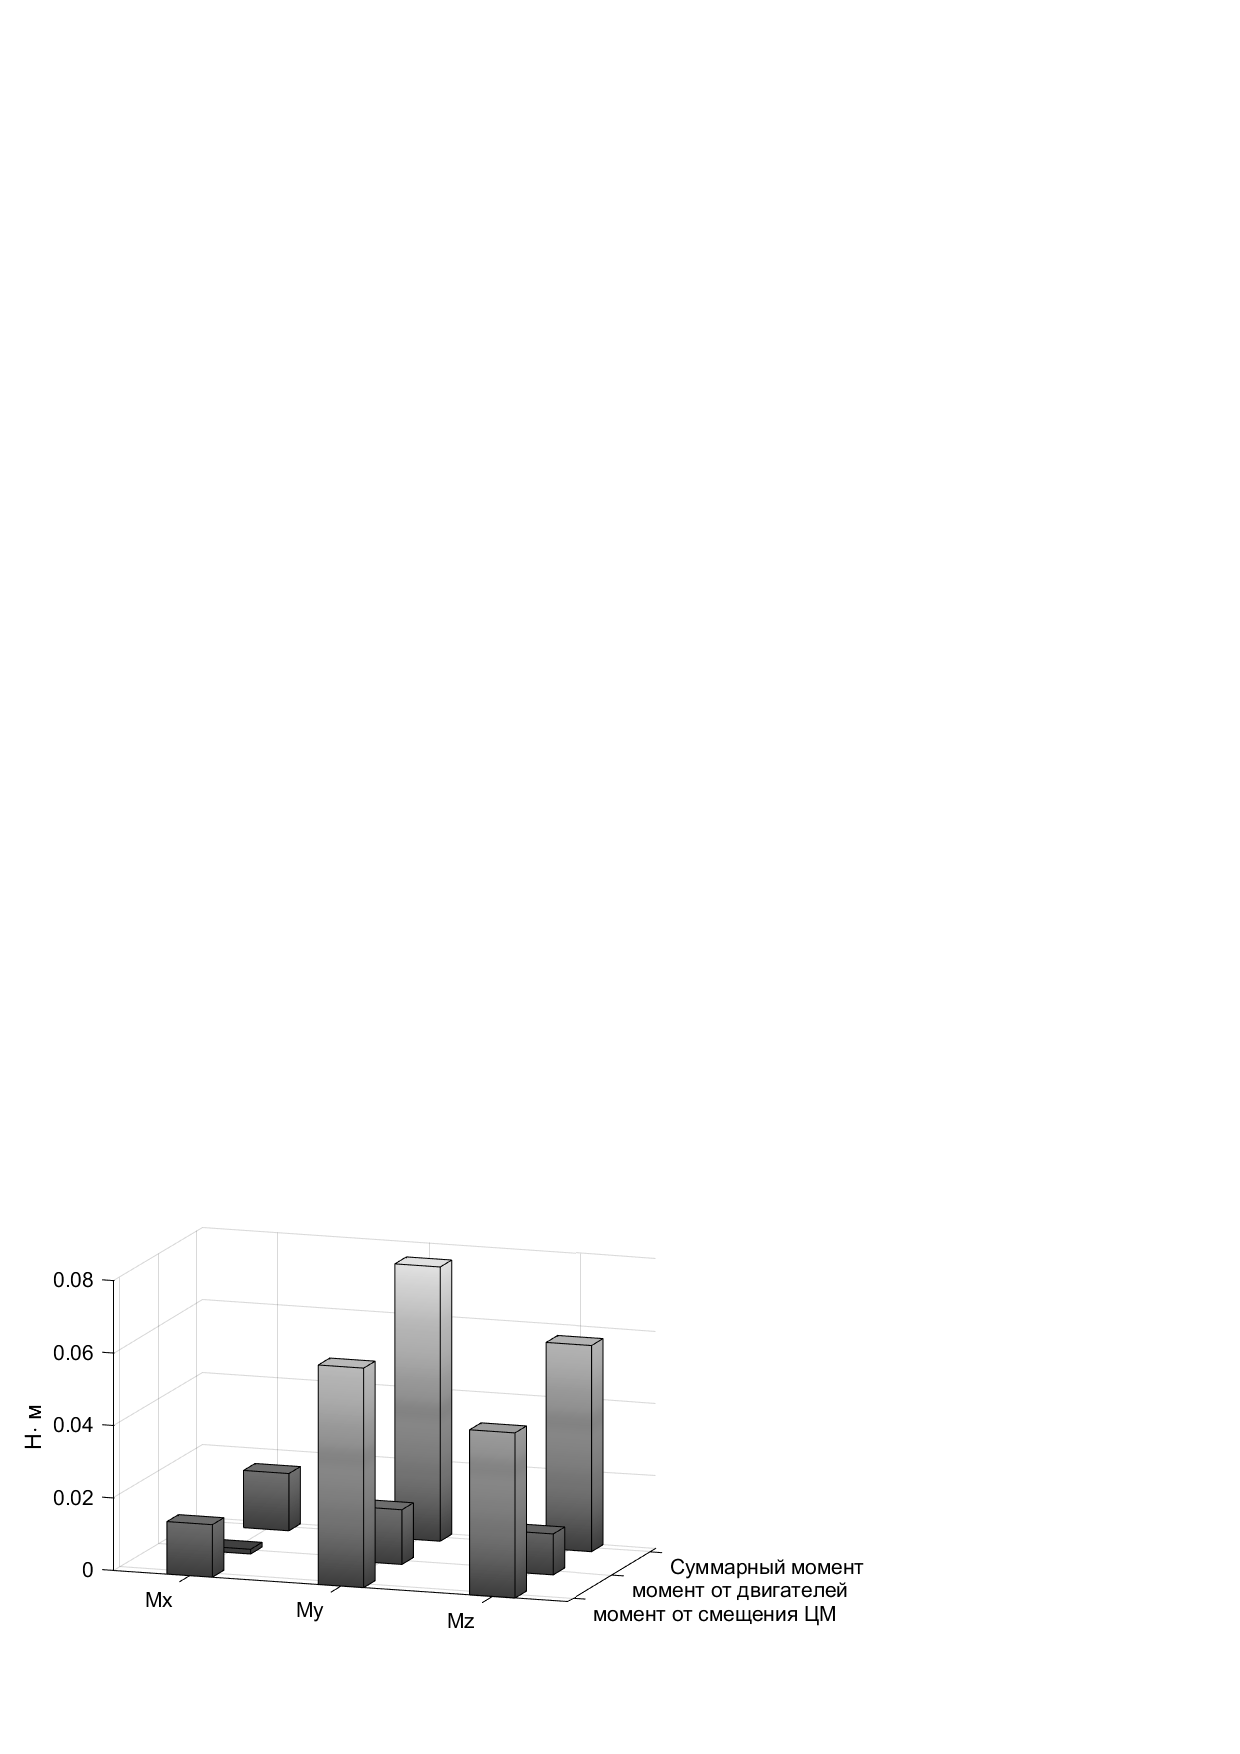
\includegraphics[scale=0.7]{matlab/moments_chart.pdf}}
	
	\caption{Распределение моментов по осям $Mx$, $My$, $Mz$ для различных источников воздействия: смещения центра масс, действия двигателей и их суммарного эффекта}
	\label{fig:momentBars}
\end{figure}

На рисунке ~\cref{fig:momentBars} приведено графическое изображение полученных результатов.

Таким образом, при заданных параметрах основной вклад в реактивные моменты вносит смещение центра карданова подвеса относительно центра масс КА, поэтому при компоновке КА указанное смещение должно быть минимизировано.

Итак, на основании изложенного можно сделать вывод о том, что максимальные реактивные моменты, действующие на основание со стороны редукторных приводов во время их функционирования, для представленного набора исходных данных не превышают величину 0,1 \si{\newton\metre}.  Основной вклад в эти моменты вносят составляющие, возникающие от наличия смещения центра карданова подвеса УПК относительно центра масс КА.

С помощью добавочных колец можно подобрать моменты инерции маховиков с целью уменьшения влияния реактивных моментов на КА.








\section{Выбор профиля разгона}

Оптические системы космического наблюдения нуждаются в высокоточных системах управления движением. Для обеспечения требуемого качества изображения и точности сопровождения предъявляются жёсткие требования — ошибка должна находиться в пределах долей угловой секунды, что соответствует современным требованиям к прецизионному наведению. Такой уровень точности должен сохраняться во всём диапазоне рабочих режимов — от малых скоростей до угловых скоростей порядка нескольких градусов в секунду. При этом механическая структура наблюдательных платформ характеризуется наличием низкочастотных собственных колебательных мод, возбуждение которых приводит к остаточным вибрациям и усложняет задачу проектирования системы управления. Одним из эффективных способов снижения динамических нагрузок и подавления возбуждения собственных мод является выбор профиля разгона привода, от которого напрямую зависят величина реактивных моментов и спектральный состав возмущающих воздействий.

Одним из ключевых факторов, определяющих величину динамических нагрузок и реактивных моментов, является закон разгона и торможения привода. Выбор профиля разгона напрямую влияет как на возмущающие воздействия на корпус аппарата, так и на точность стабилизации линии визирования. В настоящей работе рассматриваются и сравниваются несколько типов профилей разгона, на основе которых обосновывается выбор оптимального алгоритма управления.




\section{Трапецеидальный профиль разгона}
Одним из наиболее широко применяемых на практике является трапецеидальный закон изменения скорости, при котором движение подвижного узла разбивается на три участка: участок разгона с постоянным угловым ускорением, участок установившейся скорости и участок торможения с постоянным угловым замедлением. Подобный алгоритм прост в реализации и обеспечивает заданное время перемещения при минимальных требованиях к вычислительным ресурсам системы управления~\cite{Zhang2012, Austin2005}. Трапецеидальный профиль представлен на рисунке~\cref{fig:line-profile}. 

\begin{figure}[h!]
	\centering
	\includegraphics[scale=0.3]{matlab/img/line_profile.png}
	\caption{Трапецеидальный профиль разгона: зависимости ускорения, скорости и угла поворота от времени}
	\label{fig:line-profile}
\end{figure}


Математически угловая скорость при трапецеидальном профиле описывается кусочно-линейной функцией:

\begin{equation}
	\begin{split}
		\label{eq:trap_alpha}
		\alpha(t) = 
		\begin{cases}
			+\alpha_{\max}, & 0 \leq t < t_{\mathrm{acc}},\\[6pt]
			0, & t_{\mathrm{acc}} \leq t < t_{\mathrm{acc}} + t_{\mathrm{const}},\\[6pt]
			-\alpha_{\max}, & t_{\mathrm{acc}} + t_{\mathrm{const}} \leq t \leq T.
		\end{cases}
	\end{split}
\end{equation}

где \(t_{\mathrm{acc}}=\frac{\omega_{\mathrm{max}}}{\alpha_{\max}}\)"--- время разгона, \(t_{\mathrm{const}}\)"--- время движения с постоянной скоростью, \(T\)"--- общее время манёвра.

Угловая скорость изменяется по закону:

\begin{equation}
	\begin{split}
		\label{eq:trap_omega}
		\omega(t) =
		\begin{cases}
			\alpha_{\max} t, & 0 \leq t < t_{\mathrm{acc}},\\[6pt]
			\omega_{\max}, & t_{\mathrm{acc}} \leq t < t_{\mathrm{acc}} + t_{\mathrm{const}},\\[6pt]
			\omega_{\max} - \alpha_{\max}\!\bigl(t - t_{\mathrm{acc}} - t_{\mathrm{const}}\bigr), 
			& t_{\mathrm{acc}} + t_{\mathrm{const}} \leq t \leq T.
		\end{cases}
	\end{split}
\end{equation}



Угол перемещения вычисляется по выражению:

\begin{equation}
	\begin{split}
		\label{eq:theta_function}
		\theta(t) =
		\begin{cases}
			\frac{1}{2}\alpha_{\max} t^{2}, & 0 \leq t < t_{\mathrm{acc}},\\[6pt]
			\frac{1}{2}\alpha_{\max} t_{\mathrm{acc}}^{2} + \omega_{\max}(t - t_{\mathrm{acc}}), 
			& t_{\mathrm{acc}} \leq t < t_{\mathrm{acc}} + t_{\mathrm{const}},\\[6pt]
			\Delta\theta - \frac{1}{2}\alpha_{\max}(T - t)^{2}, 
			& t_{\mathrm{acc}} + t_{\mathrm{const}} \leq t \leq T.
		\end{cases}
	\end{split}
\end{equation}

где \(\Delta \theta\)"--- полный угол перемещения.


В случае, когда полный угол поворота $\Delta \theta$ мал и не удовлетворяет условию наличия участка постоянной скорости:

\begin{equation}
	\Delta \theta < \frac{\omega_{\max}^2}{\alpha_{\max}}
\end{equation}

трапецеидальный закон вырождается в треугольный профиль (Рисунок~\cref{fig:triangle_profile}). 

\begin{figure}[h!]
	\centering
	\includegraphics[scale=0.3]{matlab/img/triangle-profile.png}
	\caption{Треугольный профиль разгона как частный случай трапецеидального}
	\label{fig:triangle_profile}
\end{figure}

В этом режиме участок установившейся скорости отсутствует, а разгон сразу переходит в торможение. Максимальная скорость при этом равна:

\begin{equation}
	\omega_{\mathrm{max}} = \sqrt{\alpha_{\max}  \Delta \theta},
\end{equation}

а времена разгона и торможения составляют:

\begin{equation}
	t_{\mathrm{acc}} = t_{\mathrm{dec}} = \frac{\omega_{\mathrm{max}}}{\alpha_{\max}}, \quad T = 2t_{\mathrm{acc}}.
\end{equation}




Таким образом, трапецеидальный и треугольный профили могут быть описаны единым математическим аппаратом, различаясь лишь наличием или отсутствием участка постоянной скорости.

Реактивный момент, действующий на корпус космического аппарата, определяется как:

\begin{equation}
	M(t) = J \alpha(t),
\end{equation}

где \(J\)"--- момент инерции подвижного узла.
Для трапецеидального профиля момент принимает постоянные значения $\pm J \alpha$ на фазах разгона и торможения и равен нулю на участке установившейся скорости. 

Следует отметить, что переходы между участками профиля связаны с мгновенными скачками ускорения. В теории движения это характеризуется величиной рывка, определяемой как производная ускорения по времени:

\begin{equation}
	j(t) = \frac{d\alpha(t)}{dt}.
\end{equation}

Для идеализированного трапецеидального закона рывок представляет собой дельта-функцию в моменты переключений $t=0$, $t=t_{\mathrm{acc}}$, $t=t_{\mathrm{acc}}+t_{\mathrm{const}}$.  Именно наличие этих мгновенных скачков приводит к появлению широкополосных гармоник в спектре реактивного момента и возбуждению резонансов конструкции.

Таким образом, трапецеидальный профиль отличается простотой реализации и временем-оптимальностью при заданных ограничениях на ускорение и скорость. Однако его главный недостаток заключается в наличии рывков, вызывающих резонансное возбуждение элементов конструкции и ухудшение характеристик качества изображения в оптико-электронных системах. В связи с этим в задачах, где требуется минимизация возмущающих воздействий и подавление остаточных колебаний, целесообразно рассматривать более плавные законы изменения скорости, такие как экспоненциальный или синусоидальный.


\section{Алгоритм экспоненциального разгона}
Альтернативой трапецеидальному закону является экспоненциальный профиль изменения скорости, обеспечивающий более плавное изменение ускорения на начальном и конечном интервалах. В отличие от трапецеидального профиля, где ускорение скачкообразно изменяется, экспоненциальный закон характеризуется постепенным нарастанием и убыванием скорости, что уменьшает возбуждение высокочастотных колебательных мод конструкции~\cite{Zeng2016,Chen2008}.

Графическое представление профиля разгона показано на рис.~\ref{fig:exp_profile}.

\begin{figure}[h!]
	\centering
	\includegraphics[scale=0.8]{matlab/img/exp-profile.png}
	\caption{Экспоненциальный профиль разгона}
	\label{fig:exp_profile}
\end{figure}



Общий вид зависимости угловой скорости можно записать как:

\begin{equation}
	\label{eq:exp_speed}
	\omega(t) = \omega_{\max}\left(1 - e^{-\beta t}\right), \quad 0 \leq t \leq t_{\mathrm{acc}},
\end{equation}

где \(\beta\)"--- коэффициент сглаживания, определяющий скорость нарастания профиля. 

На участке торможения используется симметричная функция:

\begin{equation}
	\label{eq:omega_exp}
	\omega(t) = \omega_{\max} \cdot e^{-\beta \bigl(t - t_{\mathrm{acc}} - t_{\mathrm{const}}\bigr)}, 
	\qquad t_{\mathrm{acc}} + t_{\mathrm{const}} \leq t \leq T.
\end{equation}

Ускорение находится как производная от скорости:

\begin{equation}
	\label{eq:alpha_exp}
	\alpha(t) = \beta \cdot \omega_{\max} \cdot e^{-\beta t}.
\end{equation}

Угол поворота вычисляется интегрированием скорости:

\begin{equation}
	\label{eq:theta_exp}
	\theta(t) = \int \omega(t)\, dt 
	= \omega_{\max} \left( t + \frac{1}{\beta} e^{-\beta t} \right).
\end{equation}




\section{Алгоритм синусоидального разгона}

В космических приложениях наибольшую эффективность демонстрирует синусоидальный профиль разгона, поскольку он обеспечивает не только непрерывность угловой скорости и ускорения, но и плавность изменения рывка. В отличие от трапецеидального или экспоненциального закона, синусоидальный алгоритм исключает резкие скачки ускорения и тем самым существенно снижает возбуждение собственных колебательных форм конструкции, минимизируя передачу динамических нагрузок на основание и чувствительные элементы космического аппарата.

Актуальность подобных решений определяется высокими требованиями к точности сопровождения: в системах оптической спутниковой связи и космического наблюдения необходима стабилизация линии визирования в пределах долей угловой секунды при скоростях от состояния покоя до нескольких градусов в секунду~\cite{Hemmati2011,Kaushal2017}. В литературе сообщается, что современные системы слежения достигают RMS-ошибок сопровождения от $0,"$ до $2,4"$ в зависимости от архитектуры и применяемых алгоритмов управления~\cite{Park2012,Zhang2012,Riesing2017}. Достижение такого уровня точности возможно лишь при минимизации возмущающих воздействий, что, в частности, обеспечивается выбором оптимального профиля разгона привода.

Подобный закон движения рекомендуется в задачах высокоточной стабилизации и сопровождения, где требуется эффективное подавление микровибраций и сохранение качества оптических наблюдений.

Рассмотрим манёвр с углом поворота $\Delta \theta$ за время $T$ при ограничениях на максимальный скорость, ускорения и рывок:

\begin{equation}
	\label{eq:restrictions}	
	|\omega(t)| \leq \omega_{max} \quad |\epsilon(t)| \leq \epsilon_{max} \quad |j(t)| \leq j_{max}
\end{equation}

Ускорение на всём интервале $t \in [0, T]$ задаётся гармоническим законом:

\begin{equation}
	\epsilon(t) = \epsilon_0 \sin\!\left(\frac{2 \pi t}{T}\right)
\end{equation}

Тогда:

\begin{equation}
	\begin{aligned}
		\omega(t) &= \int_{0}^{t} \epsilon(\tau)\, d\tau
		= \frac{\epsilon_0 T}{2 \pi} \!\left( 1 - \cos \frac{2 \pi t}{T} \right),
		&\quad \omega(0) = \omega(T) = 0, \\[6pt]
		\theta(t) &= \int_{0}^{t} \omega(\tau)\, d\tau
		= \frac{\epsilon_0 T}{2 \pi} \!\left( t - \frac{T}{2 \pi} \sin \frac{2 \pi t}{T} \right),
		&\quad \theta(0) = 0,\ \theta(T) = \Delta \theta
	\end{aligned}
\end{equation}


Из условия $\theta(T) = \Delta \theta$ получаем амплитуду ускорения:

\begin{equation}
	\epsilon_{0} = \frac{2 \pi \Delta \theta}{T^{2}}
\end{equation}

Удобно перейти к нормированному времени $\tau=t/T \in [0,1]$. Такой переход позволяет рассматривать движение в безразмерной форме, сводя весь период к единичному интервалу (Рисунок~\cref{fig:sin-profile}). Это упрощает анализ и делает уравнения универсальными, не зависящими от конкретного значения времени манёвра:

\begin{equation}
	\begin{aligned}
		\theta(\tau) &= \Delta \theta \!\left( \tau - \frac{1}{2 \pi} \sin 2 \pi \tau \right) \\
		\omega(\tau) &= \frac{2 \Delta \theta}{T} \sin^{2} \pi \tau \\
		\epsilon(\tau) &= \frac{2 \pi \Delta \theta}{T^{2}} \sin 2 \pi \tau \\
		j(t) &= \frac{d \epsilon}{d t} = \frac{4 \pi^{2} \Delta \theta}{T^{3}} \cos\!\left(2 \pi \tau\right)\\
	\end{aligned}
\end{equation}

\begin{figure}[h!]
	% --- Первая строка ---
	\begin{minipage}[b]{0.49\linewidth}\centering
		\includegraphics[width=\linewidth]{matlab/img/theta_sin} \\ а) Угол поворота $\theta(t)$
	\end{minipage}
	\hfill
	\begin{minipage}[b]{0.49\linewidth}\centering
		\includegraphics[width=\linewidth]{matlab/img/omega_sin} \\ б) Угловая скорость $\omega(t)$
	\end{minipage}
	
	\vspace{0.5em} % расстояние между строками
	
	% --- Вторая строка ---
	\begin{minipage}[b]{0.49\linewidth}\centering
		\includegraphics[width=\linewidth]{matlab/img/eps_sin} \\ в) Угловое ускорение $\epsilon(t)$
	\end{minipage}
	\hfill
	\begin{minipage}[b]{0.49\linewidth}\centering
		\includegraphics[width=\linewidth]{matlab/img/jerk_sin} \\ г) ) Рывок $j(t)$
	\end{minipage}
	
	\caption{Параметры синусоидального профиля движения}
	\label{fig:sin-profile}
\end{figure}

Максимальные значения динамических параметров для синусоидального профиля выражаются через угол поворота и $\Delta \theta$ и длительность манёвра $T$:

Из этих соотношений следует, что сокращение периода $T$ вызывает резкий рост динамических нагрузок: скорость масштабируется как $1/T$, ускорение — как $1/T^2$, а рывок — как $1/T^3$. Таким образом, выбор длительности манёвра и формы профиля напрямую определяет уровень возбуждаемых колебаний и передаваемых нагрузок на конструкцию.

\subsection{Критерий оптимальности}

В работе выбран синусоидальный профиль разгона, поскольку при фиксированном времени манёвра $T$ он минимизирует высокочастотные гармоники ускорения в строгом смысле минимизирует энергию рывка на единицу ускорения. Формально это выражается минимумом отношения Релея:
\begin{equation}
	\label{eq:relay}
	\mathcal{R}[\epsilon] =
	\frac{\displaystyle \int_{0}^{T} \bigl(\dot{\epsilon}(t)\bigr)^{2}\,dt}
	{\displaystyle \int_{0}^{T} \epsilon^{2}(t)\,dt}
	\end{equation}

при граничных условиях:

\begin{equation}
	\epsilon(0) = \epsilon(T) = 0, \qquad
	\int_{0}^{T} \epsilon(t)\,dt = 0 \quad
	\bigl(\omega(T) - \omega(0) = 0\bigr)
\end{equation}

Любую допустимую $f(t) \in H_0^1(0,T)$ разложим в ряд по синусам:

\begin{equation}
	\epsilon(t) = \sum_{n=1}^{\infty} a_{n} \sin\!\left(\frac{n \pi t}{T}\right)
\end{equation}

Подставляя это разложение в функционал Рэлея~\cref{eq:relay}, получаем:

\begin{equation}
	\mathcal{R}[\epsilon] =
	\frac{\displaystyle \sum_{n=1}^{\infty} a_n^2 \left(\frac{n \pi}{T}\right)^2 \frac{T}{2}}
	{\displaystyle \sum_{n=1}^{\infty} a_n^2 \frac{T}{2}}
	=
	\frac{\sum_{n=1}^{\infty} a_n^2 \left(\frac{n \pi}{T}\right)^2}
	{\sum_{n=1}^{\infty} a_n^2}.
\end{equation}

Таким образом, отношение Рэлея принимает значения, ограниченные снизу наименьшим собственным значением $\lambda_n =(n\pi/T)^2$. Минимум достигается тогда, когда в разложении остаётся лишь одно слагаемое, соответствующее наименьшему допустимому $n$. Однако из условия $\int_{0}^{T} \epsilon(t)\,dt = 0$ исключаются нечётные гармоники (так как их интеграл отличен от нуля), первой подходящей собственной функцией оказывается синус с удвоенной частотой:

\begin{equation}
	\epsilon(t) = \epsilon_0 \sin\left(\frac{2\pi t}{T}\right).
\end{equation}

Следовательно, именно этот профиль ускорения реализует минимум функционала Рэлея. С практической точки зрения это означает, что синусоидальный закон обеспечивает наиболее гладкое изменение ускорения и рывка: спектр возмущающих воздействий ограничен одной основной гармоникой, а возбуждение высокочастотных колебательных мод конструкции минимально. Это напрямую приводит к снижению уровня микровибраций.

\subsection{Реализация синусоидального профиля}

Для практической реализации синусоидального закона движения был разработан алгоритм управления шаговым электроприводом, выполненный на базе микроконтроллера. Силовая часть представляет собой схему с двумя Н-мостами, позволяющая напрямую управлять токами в фазах двигателя. Такой подход обеспечит возможность формирования квазисинусоидальных токов, согласованных с теоретическим профилем разгона~\cite{Athani1997}.

Шаговый двигатель имеет две фазы --- $A$ и $B$, каждая из которых запитана через отдельный H-мост. Микроконтроллер формирует управляющие сигналы для транзисторов с помощью широтно-импульсной модуляции (ШИМ). Изменяя коэффициент заполнения ШИМ, можно регулировать среднее напряжение на обмотке, и как следствие, ток, протекающий через неё~\cite{Virgala2015}. Благодаря индуктивности обмоток ток сглаживается и повторяет заданное значение. Для формирования вращающегося магнитного поля в фазах создаются токи, сдвинутые на 90 градусов: 

\begin{equation}
	\label{eq:current_setpper}
	I_{A}(t) = I_{max} \sin(\alpha (t)) \quad I_{B}(t) = I_{max} \cos (\alpha (t))
\end{equation}

где \(I_{\max}\)"--- амплитуда тока, \(\alpha(t)\)"--- электрический угол.

В результате вектор магнитной индукции вращается равномерно, а развиваемый момент остаётся практически постоянным.

Ключевым параметром управления является электрический угол, который определяет фазу вращающегося поля. Он связан с механическим углом поворота ротора через коэффициент пересчёта, зависящий от числа шагов двигателя на один оборот.

\begin{equation}
	\label{eq:angle_electro}
	\alpha(t) =k_\alpha \cdot \theta(t),  \quad k_\alpha = \frac{N_{fs}}{4} = \frac{200}{4} = 50
\end{equation}

где \(N_{fs}\)"--- число полных шагов двигателя на один оборот. При каждом полном шаге электрический угол изменяется на четверть периода. Это означает, что при движении ротора на небольшой механический угол --- токи в фазах должны пройти заметный участок синусоиды.

Микроконтроллер вычисляет требуемую траекторию движения в соответствии с синусоидальным профилем разгона и торможения. На каждом дискретном шаге времени он обновляет текущее значение ускорения $\epsilon(t)$, скорости $\omega(t)$ и угла $\theta(t)$:

\begin{equation}
	\begin{aligned}
		\epsilon(t) &= \epsilon_0 \sin\!\left(\frac{2 \pi t}{T}\right), \\
		\omega(t + \Delta t) &= \omega(t) + \epsilon(t)\,\Delta t, \\
		\theta(t + \Delta t) &= \theta(t) + \omega(t)\,\Delta t
	\end{aligned}
\end{equation}


На основе значения $\theta(t)$ вычисляется электрический угол $\alpha(t)$, который определяет, какие значения синуса и косинуса необходимо задать для токов в обмотках. Чтобы не тратить ресурсы процессора на вычисление тригонометрических функций, в памяти контроллера хранится таблица значений синуса. Текущий электрический угол используется как адрес в таблице, и таким образом быстро извлекаются нужные значения для фазовых токов.

Полученные значения $I_A$ и $I_B$ пересчитываются в коэффициенты заполнения ШИМ. Эти коэффициенты записываются в регистры таймера, который управляет транзисторами Н-мостов. В результате в обмотках формируются токи с требуемой амплитудой и фазой.

Таким образом, управление шаговым двигателем реализовано как процесс формирования вращающегося токового вектора, скорость вращения которого изменяется в соответствии с заданным профилем движения. В отличие от традиционного пошагового режима, где момент изменяется ступенчато, предложенный метод обеспечивает плавное нарастание и спад момента, снижает вибрации и улучшает динамику системы.


\section*{Выводы по главе 2}
Во второй главе рассмотрено влияние алгоритма управления приводами и привода на величину некомпенсированных реактивных моментов, возникающих при перенацеливании оптико-механических систем. Показано, что реактивные моменты формируются за счёт двух основных факторов: смещения центра карданова подвеса относительно центра масс космического аппарата и неполной компенсации моментов двигателей маховиками. Полученные аналитические выражения позволяют раздельно оценить вклад каждой из этих составляющих. Численный пример показал, что при заданных параметрах максимальные значения реактивных моментов не превышают 0,1 Н·м, при этом наибольший вклад вносят составляющие, вызванные смещением центра подвеса относительно центра масс аппарата. Показано, что использование редукторной связи между приводом и маховиком обеспечивает пассивную компенсацию реактивных моментов без применения отдельной системы управления и позволяет снизить массу маховика за счёт уменьшения эквивалентного момента инерции.

Особое внимание уделено выбору профиля разгона, от которого напрямую зависит спектральный состав возмущающих воздействий. Установлено, что трапецеидальный закон прост в реализации, но сопровождается рывками ускорения и возбуждением широкополосных колебаний. Экспоненциальный профиль обеспечивает более плавное изменение динамических параметров, однако требует точной настройки. Синусоидальный закон разгона продемонстрировал наилучшие характеристики: он минимизирует энергию рывка на единицу ускорения, ограничивает спектр возмущений одной гармоникой и тем самым снижает уровень микровибраций.

Таким образом, в главе показано, что величина остаточных реактивных моментов определяется не только конструктивными особенностями системы, но и выбором алгоритма управления приводами. Применение синусоидального профиля разгона совместно с корректным подбором параметров маховиков обеспечивает значительное уменьшение динамических нагрузок и минимизацию их влияния на характеристики оптико-электронных систем.





\FloatBarrier
